\documentclass[class=book, crop=false, oneside, 12pt]{standalone}
\usepackage{standalone}
\usepackage{../../style}
\graphicspath{{./assets/images/}}

\begin{document}

\chapter{provvisori(ssim)o}

\section{Analisi lessicale}
\subsection{Introduzione}
Dopo i precedenti due capitoli, nei quali abbiamo introdotto e approfondito un buono numero di concetti, algoritmi e modelli necessari alla comprensione di come l'impostazione teorica dei linguaggi formali sia fondamentale nella progettazione dei compilatori, andiamo a tuffarci in quella che è la prima fase di compilazione: l'analisi lessicale.


Ricordiamo che questa è la fase in cui vogliamo identificare quali parti del sorgente che abbiamo scritto corrispondono alle keyword, quali agli identificatori,alle costanti, e via di questo passo; per essere più formali, questi elementi che vogliamo riconoscere portano il nome di \emph{lessemi}, e trasformare quindi il sorgente in un flusso di tokens, i quali costituiscono i terminali della grammatica che genera il nostro linguaggio di programmazione.

La grammaticafi un linguaggio ci dirà quali sono le forme che un'espressione deve avere per essere considerata ben formata rispetto a quel linguaggio. Ad esempio, una grammatica ci può dire che la seguente forma denota un'espressione valida:\\
% begin minted
Identificatore      simbolo di assegnamento    numero\\
% end minted
e che quindi espressioni ome la seguente sono grammaticali e ben formate secondo il linguaggio.\\
% begin minted
pippo = 2\\
% end minted8
Il mestiere dell'analizzatore lessicale è proprio quello di ricevere in input un \texttt{pippo} qualsiasi (che è un token) e, in output, determinare che è un \emph{identificatore}, ossia la categoria più astratta (lessema) di cui \texttt{pippo} è istanza.

% L’analizzatore lessicale lavora in tandem (pipeline) con l’analizzatore sintattico per non si sa bene come o perché
\subsection{Esempio: la grammatica di C99}
Andiamo a vedere da vicino la grammatica di un reale linguaggio, anzi, del linguaggio preferito di tutti noi, ossia il C (nella versione \(99\), scritta per il parser \emph{Bison}); il lettore interessato ad approfondire può trovare lo stesso file cliccando \href{./assets/files/c99.y}{qui} (fonte: \url{http://www.quut.com/c/ANSI-C-grammar-y-1999.html}).
\begin{figure}[H]
    \centering
    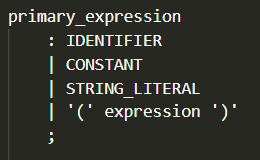
\includegraphics[width=.4\textwidth,keepaspectratio]{c99-ex1}
    \caption{}
    % \label{dfa-b_odd-and-a_even}
\end{figure}
Notiamo subito alcune differenze rispetto alla notazione che abbiamo impiegato finora: 
\begin{itemize}
    \item la freccia ( \(\to\) ) è rappresentata da un altro simbolo, i due punti ( \(:\) );
    \item il pipe ( \(\mid\) ), invece, possiede il medesimo significato;
    \item i terminali possono essere indicati precisamente con '';
    \item inoltre, la convenzione rispetto alla capitalizzazione è invertita: qui osserviamo che gli elementi in maiuscolo sono i terminali, mentre invece quelli in minuscolo rappresentano non terminali; ad esempio, in figura sopra possiamo notare che il non-letterale \texttt{primary\_expression} ha una produzione per cui può risultare o in una serie di letterali (\texttt{IDENTIFIER}, \texttt{CONSTANT}), oppure in una forma \texttt{'(' expression ')'}, dove \texttt{expression} è un altro non letterale, che a sua volta avrà altre produzioni.
\end{itemize}

Questo file, inoltre, è pensato per essere utilizzato in tandem con un analizzatore sintattico; per questo motivo, nell'intestazione dello stesso possiamo trovare le dichiarazione di quelli che sono i token (vale a dire, lo ripetiamo, i terminali della grammatica descritta). Saranno espressi in questa forma:
\begin{figure}[H]
    \centering
    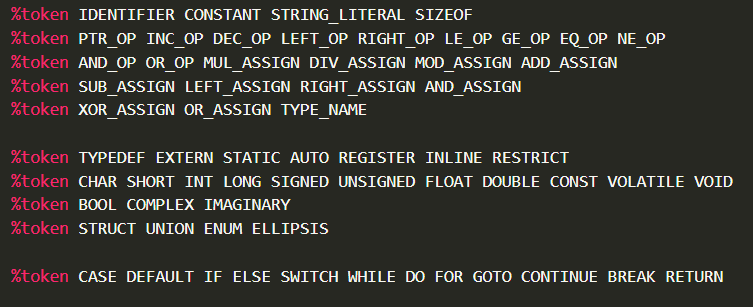
\includegraphics[width=.7\textwidth,keepaspectratio]{c99-ex2}
    \caption{}
    % \label{dfa-b_odd-and-a_even}
\end{figure}

Un'altra cosa che possiamo osservare è la dichiarazione di quello che è lo starting symbol della grammatica:\\
% begin minted
\% start translation\_unit\\
% end minted
Questa dichiarazione in realtà potrebbe non essere presente su alcuni file contenenti grammatiche, dal momento che, in sua assenza, non otteniamo degli errori, bensì viene preso il non-letterale della prima produzione listata a seguito come starting symbol.

Il ruolo dell’analizzatore lessicale è quindi analizzare il sorgente e decidere, di volta in volta, quale derivazione può essere applicata a ciascuna delle righe del sorgente analizzato. Una volta completato l'albero di derivazione e quindi arrivato presso un terminale (ad esempio \texttt{IDENTIFIER}), l'analizzatore lessicale andrà anche ad associargli un valore, dal momento che è necessario distinguere quell'\texttt{IDENTIFIER} da un altro; questo è necessario, perché nel programma potremmo tranquillamente avere due \texttt{IDENTIFIER} di diverso tipo, o in ogni caso potremmo comunque voler conservare delle informazioni aggiuntive di qualche tipo (nome, scope e altro ancora). Tutte queste informazioni vengono conservate in una \emph{symbol table}.

Infine, le ultime rihe del file contengono informazioni utili al particolare analizzatore sintattico utilizzato; avremo modo di parlarne nel dettaglio in futuro.

\subsection{Classi di tokens}
Si potrebbe a ragione considerare superfluo specificare che ogni diversa grammatica (e quindi ogni linguaggio) presenta diverse categorie di tokens; banalmente, il lettore è probabilmente ben cosciente che linguaggi diversi possiedono generalmente keyword diverse. Ad ogni modo, a seguito presentiamo alcune tra le scelte più ricorrenti:
\begin{itemize}
    \item un token per ogni keyword, quindi un token per ogni nome di base già presente nel linguaggio (\texttt{if}, \texttt{while}, \texttt{for} e via dicendo;
    \item un token per ogni operatore (o anche per classe di operatori), quindi in C ne avremo uno per \texttt{+} ma anche uno dedicato per \texttt{++}; 
    \item un unico token per gli identificatori, valido per tutti quanti;
    \item un token per ogni simbolo di punteggiatura. 
\end{itemize}

\subsection{Il lavoro dell'analizzatore lessicale}
L'obiettivo dell'analalizzatore lessicale è quindi riconoscere i cosiddetti \emph{lessemi}, ossia quelle parti del programma che corrispondono ai token, e ritornarli. Ciascuno di questi, di solito, vengono ritornati sotto forma di coppia \texttt{<token-name>: <token-value>}, dove:
\begin{itemize}
    \item \texttt{<token-name>} è il nome scelto per denotare quel preciso token; seguendo l'esempio della grammatica precedente, \texttt{IDENTIFIER} è un \texttt{<token-name>};
    \item \texttt{<token-value>} è tipicamente un puntatore a una entry della symbol table, in cui si va a salvare tutte le informazioni relative a quel preciso token di tipo\footnote{In questo caso la parola "tipo" è chiaramente impropria, ma è molto utile per rendere la natura astratta di classe di token.} \texttt{<token-name>}.
\end{itemize}

\subsection{Lessemi e espressioni regolari}
Andiamo quindi a capire in che modo la teoria studiata nei due capitoli precedenti entra prepotentemente nell'analisi lessicale.

I lessemi sono estremamente facili da descrivere utilizzando le espressioni regolari: ad esempio, in un linguaggio che prevede un lessema identificatore, il quale è costituito di qualsiasi combinazione di lettere maiuscole e minuscole, quest'ultimo può essere facilmente denotato da un'espressione regolare del tipo:
\begin{equation*}
    (a \mid b \mid \ldots \mid z \mid A \mid B \mid \ldots \mid Z)^*
\end{equation*}
Questo è molto interessante: se è vero che i lessemi sono perfettamente descrivibili con dei linguaggi regolari, allora vuol dire che possiamo utilizzare quelli in sede di analisi lessicale, senza dover tirare in ballo i più potenti ma decisamente più complessi linguaggi liberi.

Quindi questi lessemi, essendo descritti da delle espressioni regolari, possono anche essere riconosciuti agevolmente da una macchina a stati, come ad esempio quella in figura sotto, che descrive la classe \texttt{relop} di token per gli operatori relazionali.
\begin{figure}[H]
    \centering
    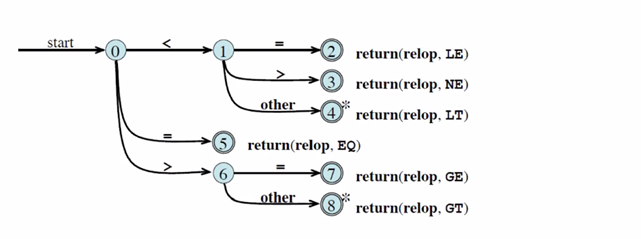
\includegraphics[width=\textwidth,keepaspectratio]{lec-14-1}
    \caption{}
    % \label{dfa-b_odd-and-a_even}
\end{figure}
È molto semplice intuire graficamente che ciascun percorso che termini in uno stato finale ritorna un token, sotto forma di coppia, in cui il \texttt{token-name} è appunto quello della classe \texttt{relop}, mentre il \texttt{token-value} indica qual è l'elemento della classe da ritornare.

\paragraph{Retract}
Possiamo notare che i due stati finali il cui arco entrante è marcato come \(other\) hanno anche un asterisco: questo indica che, quando consumo quella transizione, devo ricordarmi di tornare indietro di una parola, perché quest'ultima parola \(other\) (cioè che non fa parti di alcun elemento appartenente alla classe \texttt{relop}) potrebbe essere un elemento di un token successivo, e se non compiano quanto detto sopra rischieremmo di saltarla nell'analisi e ottenere un flusso di token incorretto. Questa operazione è detta \(retract\).

L'operazione di retract è unodei tanti elementi legati alla gestione dell'input e del buffer che ci fanno pensare che la macchina a stati è un modello molto vicino al più noto, per noi, automa a stati finiti, ma quanto è profondo questo legame?

\subsection{Pattern matching basato su NFA}
Immaginiamo di avere delle espressioni regolari che denotano il linguaggio dei lessemi che siamo interessati a riconoscere. Si pensi ad esempio all'espressione regolare che denota il lessema \texttt{IDENTIFIER}, ossia l'espressione regolare che denota tutte le possibili combinazioni di lettere maiuscole e minuscole (con le dovute peculiarità di ciascun linguaggio); oppure, si pensi a un'espressione regolare che denoti il lessema degli operatori relazionali, o ancora un'altra che denoti la scrittura dei floating numbers. In sostanza, per ciascuna categoria sintattica abbiamo un'espressione regolare che la denota.

Sappiamo anche che, avendo delle espressioni regolari, per ciascuna di queste possiamo costruire degli NFA che riconoscono il linguaggio denotato dall'espressione considerata; possiamo a questo punto immaginare di far collidere questi NFA inserendo uno stato iniziale extra e collegandolo a ciascun NFA tramite una \(\varepsilon\)-transizione, come mostrato in figura sotto.
\begin{figure}[H]
    \centering
    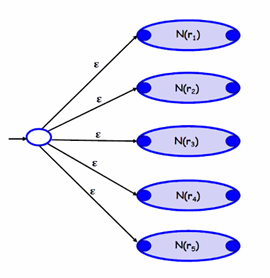
\includegraphics[width=.4\textwidth,keepaspectratio]{lec-14-2}
    \caption{}
    % \label{dfa-b_odd-and-a_even}
\end{figure}
Una struttura di questo tipo può riconoscere i linguaggi denotati da tutte le espressioni regolari per cui abbiamo costruito degli NFA. 

Adesso dobbiamo pensare come ottimizzare l'uso di una struttura simile per l'analisi lessicale. Potremmo trovarci infatti a gestire problemi di diversa natura, in particolare relativi all'input buffering: ad esempio, come posso fare a sapere se i due caratteri \texttt{i} e \texttt{f} che ho appena letto stanno a indicare la keyword \texttt{if} e non un ipotetico identificatore \texttt{iffoff}? Detto in maniera informale, come decido quando fermarmi, quando tornare indietro, quando e se ho letto più di quanto mi serviva?

Il procedimento che seguiamo è il seguente:
\begin{enumerate}
    \item innanzitutto simuliamo l'NFA creato come sopra descritto;
    \item ci sono delle azioni associate agli stati finali;
    \item nel caso di ambiguità, ossia di situazioni come quella descritta sopra tra \texttt{if}e \texttt{iffoff},  la convenzione è di preoseguire la simulazione finché nessun’altra transizione è possibile, solitamente quando incontriamo uno spazio o un \texttt{\(\backslash\)n} (si parla di cercare il \emph{longest match});
    \item se nell'insieme di stato che abbiamo raggiunto ci sono delle azioni disponibili, allora ciascuna azione avrà una priorità, e noi andremo a eseguire quella con più alta priorità;
    \item se nessun'azione è disponibile, invece dobbiamo torniamo indietro nella sequenza di stati percorsi, fermarci nel primo insieme di stati che presenta almeno uno stato finale e delle azioni associate e cercare di nuovo quella prioritaria; per ognuno di questi passi all'indietro, dobbiamo ricordari di aggiornare il puntatore all'input buffer.
\end{enumerate}

Tutto questo funziona in maniera analoga se utilizzassimo un DFA: dovremmo semplicemente costruire il DFA a partire dal NFA, dimodoché l'insieme degli stati del DFA sia un sottoinsieme di quello dell'NFA corrispondente.

\subsection{Generatori di analizzatori lessicali}
Andiamo a parlare quindi di questi generatori. L'idea di creare un generatore di analizzatori lessicali è nata in concomitanza con la prima definizione e implementazione del compilatore del C, e l'idea era di evitare di dover scrivere ogni volta, per ogni programma, un analizzatore lessicale e uno sintattico a mano.

\emph{Flex} è il primo della sua storia\footnote{o meglio, una sua versione più moderna: il primo vero e proprio si chiamava \emph{lex} e quella \emph{f}, aggiunta successivamente, sta per fast.} ed è solitamente compreso nelle distribuzioni di C; l'idea è risultata talmente valida che oggiggiorno ogni linguaggio possiede un proprio generatore di analizzatore lessiale e sintattico.

Il funzionamento è il seguente: 
\begin{itemize}
    \item andremo a creare un file del tipo \texttt{file.l}, il quale sarà l'input del generatore e in cui scriveremo quali sono i pattern che vogliamo riconoscere e quali sono le azioni da compiere in corrispondenza dei vari matches;
    \item a quel punto, possiamo comiplare \texttt{file.l} utilizzando il comando \texttt{flex}, e questo ci restituirà un file di nome \texttt{lex.yy.c}\footnote{La ragione di questo nome è puramente convenzionale e deriva dal fatto che, storicamente, il generatore flex è stato usato in coppia all'analizzatore \emph{Yacc}};
    \item compilando questo \texttt{lex.yy.c} con il compilatore \texttt{gcc} otteniamo il lexer, cioè quel signore che si occupa di gestire l'input buffering, di fare le operazioni di retract e altro ancora.
\end{itemize} 
% begin minted
flex file.l
gcc lex.yy.c -lfl
./a
% end minted
Si tenga bene a mente che queste tre righe descrivono come utilizzare flex da solo; tuttavia, quest'ultima è un'eventualità piuttosto rara, dal momento che flex è nato per essere usato in pipeline con un generatore di analizzatore di analisi sintattica, ma poiché questi sono elementi ancora sconosciuti per noi, al momento non ce ne preoccupiamo.

\subsection{Struttura del \texttt{file.l}}
I file con estensione \texttt{.l} che diamo da fagocitare a flex hanno la seguente struttura:
% begin minted
...(Preambolo)
% { code
% } %
shorthand for patterns
%%
(Parte centrale)
pattern-1 {action-1};
pattern-2 {action-2};
...
%%
(Epilogo)
user rountes
% end minted
Il contenuto di queste tre macrosezioni è ben determinato, andiamo a vederlo più da vicino:
\begin{labeling}{Parte centrale}
    \item[Preambolo] qui ci andrà del codice C,in particolare le inizializzazioni di variabili, o delle abbreviazioni per indicare dei particolari pattern nelle espressioni regolari che andremo a utilizzare sotto;
    \item[Parte centrale] è il cuore del file, e si tratta di una lista pattern-azione, dove pattern è un'espressione regolare, e l'azione sarà ciò che dobbiamo compiere qualora dovessimo riconoscere il pattern corrispondente;
    \item[Epilogo] questa sezione è in realtà facoltativa, il lexer funziona anche senza che vi sia scritto alcunché; tuttavia, quello che potremmo eventualmente trovare e/o scrivere sono delle routine definite dall'utente, le quali verranno copiate e incollate dentro al genituro \texttt{lex.yy.c}.
\end{labeling}

\subsection{Linguaggio delle espressioni regolari in flex}
Dal momento che tutte le coppie \texttt{pattern \{azione\}} sono scritte in linguaggio \texttt{lex}, a differenza di altre parti di \texttt{file.l}, è opportuno conoscere questo linguaggio. Di seguito presentiamo i \emph{metacaratteri} di flex, ossia dei caratteri riservati:
\begin{equation*}
    \slash \quad \backslash \quad - \quad * \quad + \quad >\quad " \quad \{ \quad \} \quad . \quad \$ \quad ( \quad ) \quad \mid \quad \% \quad [ \quad ] \quad ^\wedge
\end{equation*}
\noindent Andiamo a vedere più da vicino quali sono le regole di matching dei metacaratteri:
\begin{labeling}{a | b}
    \item[\texttt{.}] qualsiasi carattere, eccetto il newline;
    \item[\texttt{\(\backslash\)n}] il newline;
    \item[\texttt{*}] zero o più copie di un elemento;
    \item[\texttt{+}] una o più copie di un elemento;
    \item[\texttt{?}] zero o una copia di un elemento;
    \item[\texttt{[]}] denota le classi di caratteri: al posto di \(a \mid b \mid \ldots \mid z\), posso scrivere \texttt{[a-z]};
    \item[\texttt{\(^\wedge\)}] inizio di riga, negazione se usato in una classe di caratteri;
    \item[\texttt{\$}] end of line;
    \item[\texttt{a|b}] pipe, semantica consueta;
    \item[\texttt{()}] raggruppamenti;
    \item[\texttt{"+"}] somma letterale di due elementi
    \item[\texttt{\{\}}] espressioni regolari scritte nel preambolo
\end{labeling}

\subsection{File per FLEX}
Tutti i file predisposti per flex si compongono da tre sezioni separate da coppie di \%. Nel preambolo si inseriscono delle definizioni come le define che servono e i pattern (espressioni regolari per i lessemi che vogliamo inserire). I pattern sono inseriti insieme all'azione nella parte centrale. In fondo si inseriscono le routine dell'utente che vengono copiate nel file lex.yy.c: un testo minimale è l'invocazione della routine yylex() che se non viene inserita viene chiamata in automatico. I comandi, qualora non si usi flex con byson (analizzatore sintattico in pipeline con flex), sono
\begin{itemize}
    \item flex file.l
    \item gcc lex.yy.c lfl
    \item ./a
\end{itemize}

\subsubsection{file0.l}
        
\begin{figure}[h]
    \centering
    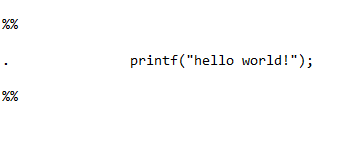
\includegraphics[width=.7\textwidth,keepaspectratio]{file0.l.png}
    \caption{file0.l}
    \label{file0.l}
\end{figure}


In qusto primo esempio non sono presenti delle define o del codice c nel preambolo e, visto che non sono presenti routine inserite dall'utente, verrà invocato il \emph{yylex()} all'esecuzione.

Basandoci sulla sintassi di FLEX vista precedentemente analizziamo la parte centrale costituita da una sola coppia pattern-azione:
\begin{itemize}
    \item il pattern è dato dalla regular expression composta solo da ., il che significa che l'azione seguente farà riferimento a tutti i caratteri incontrati tranne quello di \emph{new line}
    \item l'azione è \emph{printf("hello world!")} che consiste banalmente nello stampare hello world ogni volta che viene eseguito un match sul pattern
\end{itemize}

Il tutto si traduce nell'andare a sostituire ad ogni carattere incontrato diverso da new line un'occorrenza di hello world. In pratica ciò significa che
\begin{itemize}
    \item \(a\) diventa hello world!
    \item \(aa\) diventa hello world!hello world!
\end{itemize}

Una cosa molto interessante che è possibile notare è che solitamente per poter utilizzare lo standard output nei programmi c è necessario includere all'interno del file la libreria stdout mentre nel file0.l non vi è nemmeno l'ombra di un inlcude: è flex che si preoccupa di aggiungere in un secondo momento tutti i dettagli necessari per l'output.

\subsubsection{file1.l}

\begin{figure}[h]
    \centering
    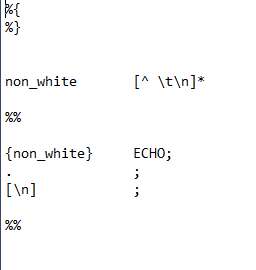
\includegraphics[width=.7\textwidth,keepaspectratio]{file1.l.png}
    \caption{file1.l}
    \label{file1.l}
\end{figure}

In questo caso osserviamo che il preambolo del file1.l non è vuoto come nel caso precedente e si compone invece di quelle che possiamo identificare come due sezioni

\begin{enumerate}
    \item la prima (in questo caso vuota) è identificata dal simbolo di apertura \%\{ e cui può seguire del codice C
    \item la seconda invece è successiva al simbolo di chiusura \%\} e contiene quelli che sono gli shorthands per i pattern, cioè degli alias per delle regular expression
\end{enumerate}

Rifacendoci sempre alla sintassi di FLEX, possiamo analizzare l'espressione regolare definita nel preambolo e arrivare alla conclusione che faccia riferimento a quell'insieme di caratteri ([ ]) che si ripetono 0 o più volte (*) e che sono diversi (\^{}) da ' ', '\textbackslash t' e '\textbackslash n': questo significa che comporteranno un match tutte quelle sequenze di caratteri che sono separate da spazi, tab o new line o, più semplicemnte, le parole.

Come descritto precedentemente nella parte centrale i pattern sono associati alle relative azioni, in questo caso
\begin{itemize}
    \item non\_white comporta l'esecuzione della macro ECHO di flex, che è equivalente a  printf ("\%s", yytext), e stamperà a video esattamente la sequenza di caratteri che ha fatto match
    \item un qualunque carattere diverso da \textbackslash n (.) verrà eliminato
    \item new line (\textbackslash n) verrà anch'esso eliminato
\end{itemize}

Complessivamente il risultato ottenuto dall'esecuzione di un programma compilato a partire dal file discusso porterà all'eliminazione di ' ', '\textbackslash t' e '\textbackslash n' dal testo passato in input e quindi ad una sequenza continua di caratteri (e.g. ab c d e      f g \emph{diventerà} abcdefg)

\subsubsection{file2.l}

\begin{figure}[h]
    \centering
    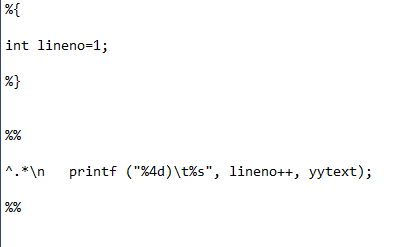
\includegraphics[width=.7\textwidth,keepaspectratio]{file2.l.png}
    \caption{file2.l}
    \label{file2.l}
\end{figure}

In questo esempio invece possiamo vedere nel preambolo la presenza di codice C compreso nel blocco indicato da \%\{ e \%\}, in particolare la dichiarazione di un intero chiamato lineno ed inizializzato al valore 1.

A seguire abbiamo la parte centrale del file dove 

\begin{itemize}
    \item all'espressione regolare \^{}.*\textbackslash n, che identifica tutte quelle sequenze di caratteri che iniziano per un carattere differente da new line ripetuto zero o più volte e finiscono per new line o, più semplicemente, le parole sulla stessa riga
    \item  viene associata l'azione printf("\%4d)\textbackslash t\%s", lineno++, yytext), che stampa il valore dell'intero lineno seguito dal simbolo ) e dal contenuto del buffer yytext (che contiene l'input fino ad ora riconosciuto) ed infine esegue il postincremento di lineno.
\end{itemize}

In sostanza dunque il programma si occuperà di stampare tutte le parole sulla stessa riga anteponendo il numero della riga a cui fa riferimento; ciò vuol dire che il seguente testo

\begin{itemize}
    \item[] \emph{Autem quo ea. Voluptatum saepe porro. Quibusdam illo eum.}

    \item[] \emph{Quia aperiam nesciunt. Qui est voluptate. Aut temporibus perspiciatis.}

    \item[] \emph{Repudiandae delectus omnis. Modi earum doloribus. Quis eaque quidem.}
\end{itemize}
verrà dunque riscritto nel seguente modo

\begin{enumerate}
    \item[1)] \emph{Autem quo ea. Voluptatum saepe porro. Quibusdam illo eum.}
    \item[2)] \emph{Quia aperiam nesciunt. Qui est voluptate. Aut temporibus perspiciatis.}
    \item[3)] \emph{Repudiandae delectus omnis. Modi earum doloribus. Quis eaque quidem.}
\end{enumerate}

\subsubsection{file3.l}

\begin{figure}[h]
    \centering
    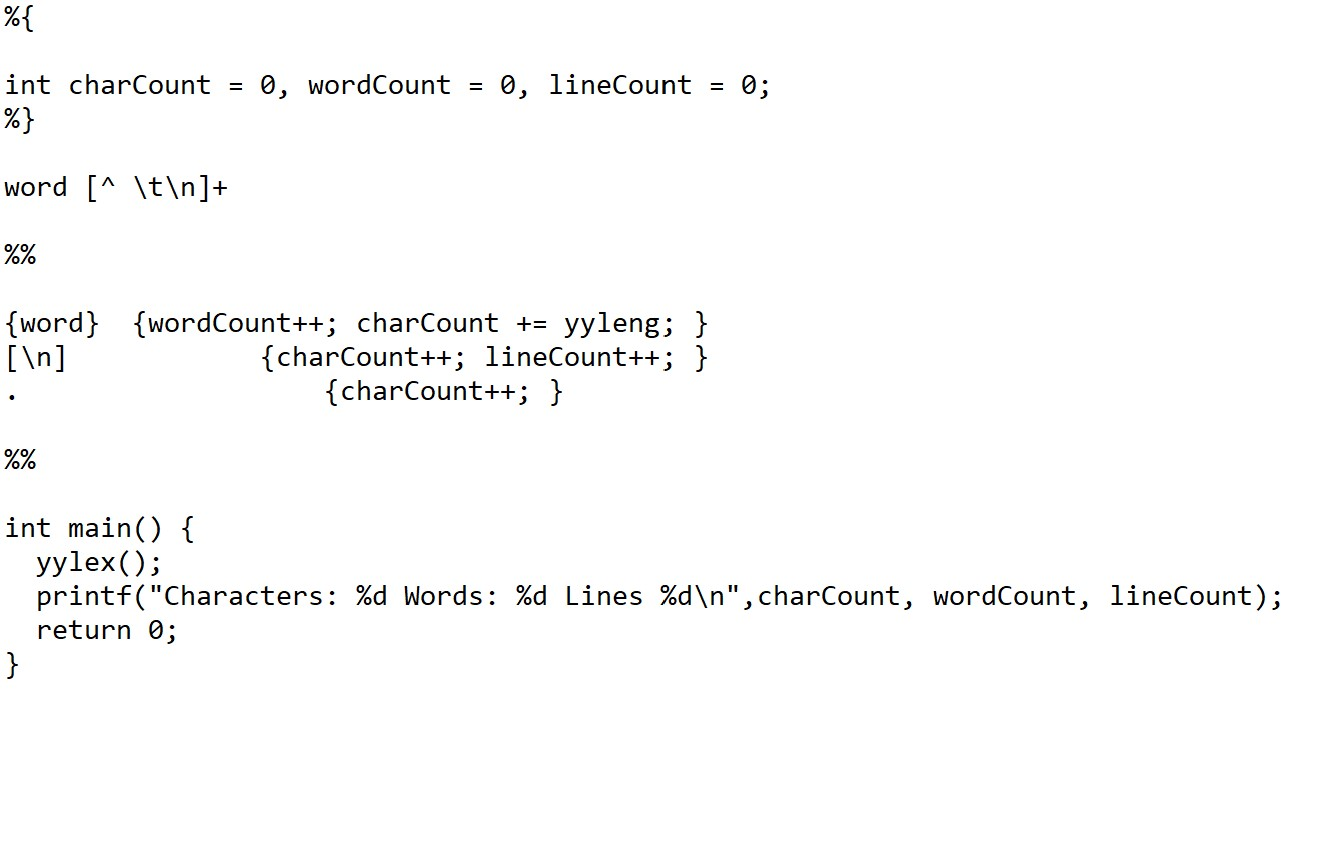
\includegraphics[width=.7\textwidth,keepaspectratio]{file3.l.jpg}
    \caption{file3.l}
    \label{file3.l}
\end{figure}

Nel quarto esempio combiniamo quanto visto precedentemente aggiungendo anche una routine custom scrivendo del codice ad hoc nell'epilogo del file.

Nel prologo abbiamo la dichiarazione di tre variabili che ci serviranno nelle routine come contatori e in più di una shorthand, chiamata word, la cui espressione regolare include tutte quelle sequenze di uno o più caratteri (+) che non contengono ' ', \textbackslash t, \textbackslash n.

Nella parte centrale del file abbiamo invece le seguenti associazioni pattern-azione, in particolare

\begin{itemize}
    \item word comporta l'esecuzione del seguente pezzo di codice \{wordCount++; charCount+=yyleng; \}, dove la variabile wordCount viene postincrementata mentre alla variabile charCount viene sommato un numero pari a yyleng, che contiene la lunghezza della stringa riconosciuta e, per via dell'espressione regolare alla base della shorthand, equivalente a quella della parola
    \item [\textbackslash n], cioè nel caso in cui si trovi una sequenza di caratteri composta solamente da una new line, è legata all'azione \{charCount++; lineCount++; \} dove si postincrementano sia charCount che lineCount
    \item . infine comporta solamente il postincremento della variabile charCount
\end{itemize}

In sostanza il programma che stiamo descrivendo mediante i pattern discussi si occupa di contare complessivamente quanti caratteri, parole e righe sono state individuate in un certo testo: nel caso di un match con una parola avviene un incremento proporzionale al numero di caratteri che la costituiscono e si aggiorna anche il numero di parole che sono contenute nel testo; ogni volta che si trova una new line si incrementano di un'unità il numero di righe oltre che al numero di caratteri; infine ogni volta che si trova uno spazio o un tab viene incrementato solamente il numero di caratteri. 

\subsubsection{file4.l}

\begin{figure}[h]
    \centering
    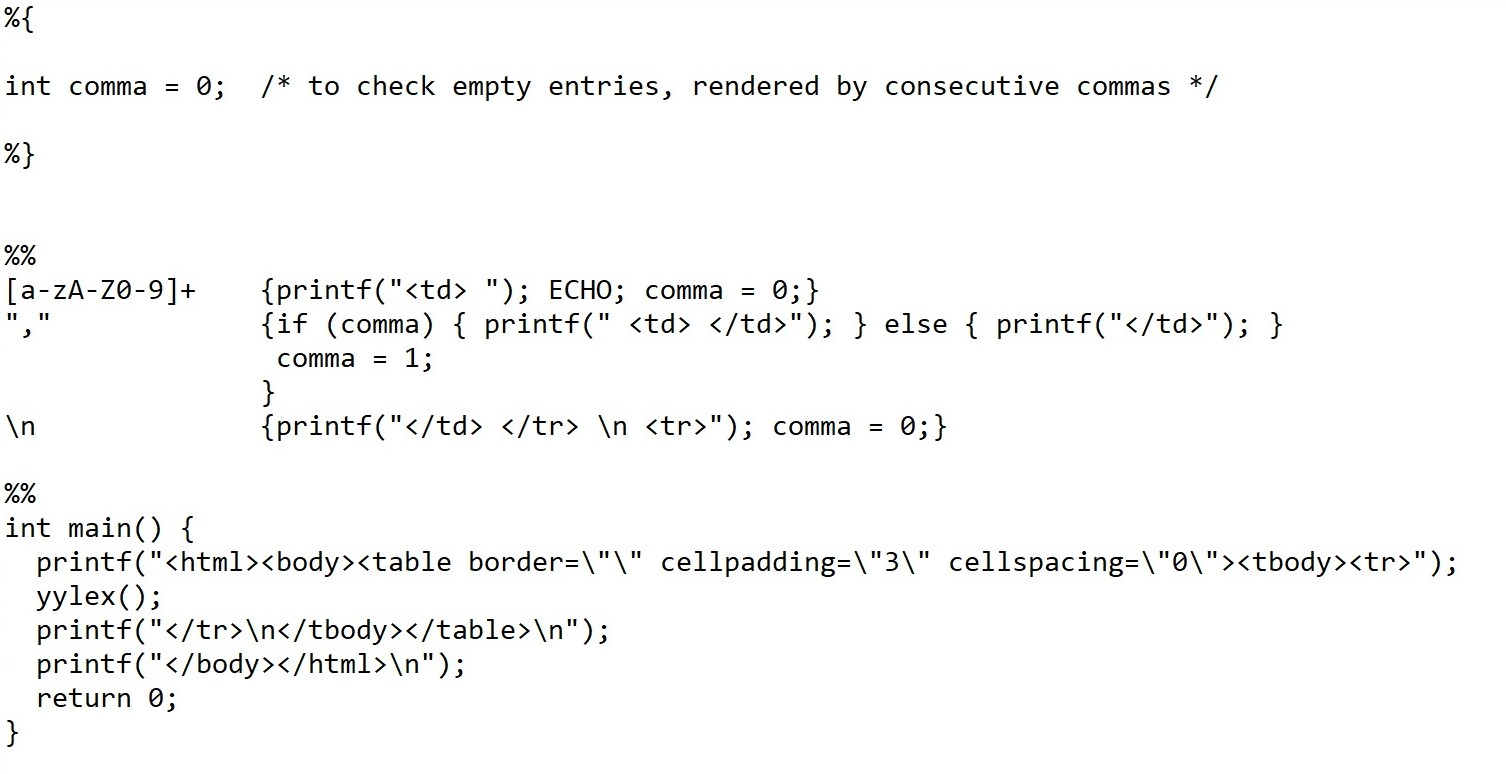
\includegraphics[width=.7\textwidth,keepaspectratio]{file4.l.jpg}
    \caption{file4.l}
    \label{file4.l}
\end{figure}

L'ultimo esempio proposto fa uso di quanto discusso fino ad ora per analizzare un csv e restituire i dati sotto forma di una tabella in formato html:

\begin{itemize}
    \item Nel preambolo viene dichiarata una variabile intera comma inizializzata a 0 che servirà per controllare le entry vuote nel csv passato in input date da virgole consecutive
    \item Nella parte centrale si hanno le seguenti coppie pattern-azione
    \begin{itemize}
        \item La regular expression [a-zA-Z0-9]+, che indica la sequenza di uno o più caratteri alfanumerici, comporta l'esecuzione di 
        
        \{printf("\(<\)td\(>\) "); ECHO; comma=0; \} 
        
        dove viene creata una nuova colonna per la tabella, viene inserita la sequenza appena letta e viene impostato il valore dell'intero comma a 0
        \item ",", cioè trovare il carattere che corrisponde alla virgola e che nel csv server per separare i dati, comporta l'esecuzione del blocco di codice
        \{
        
        if (comma) \{
        
        printf("\(<\)td\(>\) \(<\)/td\(>\)"); 
        
        \} else \{ 
        
        printf("\(</\)td\(>\)");
        
        \}
            
            comma = 1;
                 
        \}
        
        dove viene verificato il numero di virgole incontrate fino a quel punto: se si sono incontrate 0 virgole allora si chiude semplicemente la colonna precedentemente aperta; se invece si è già incontrata 1 virgola e consecutivamente se ne legge un'altra (o comunque le due occorrenze risultano essere separate da sequenze non alfanumeriche), viene creata una colonna vuota in quanto nel csv non vi sono dati rilevanti. In ogni caso alla fine del blocco viene impostato il valore di comma ad 1
        \item \textbackslash n, cioè per ogni new line, viene eseguito il blocco di codice \{printf("\(<\)/tr\(>\) \textbackslash n \(<\)tr\(>\)"); comma = 0;\} dove viene chiusa la riga precedente ed aperta quella successiva
    \end{itemize}
    \item Nell'epilogo possiamo trovare una routine custom dove viene creato l'html di base per creare la tabella e, tra le varie cose, viene anche aperta la prima riga. Dopo aver stampato lo scheletro della struttura viene invocato il \emph{yylex()} che cerca i pattern nel testo ed infine viene chiusa la tabella
\end{itemize}

\subsection{Di più relativamente a flex}
Quando abbiamo discusso del funzionamento dell'analisi lessicale basata sull'utilizzo di NFA o DFA abbiamo anche parlato del fatto che, quando si tenta di riconoscere il pattern di una determinata parola, è possibile che avvengano dei match su più stati finali dell'automa e che quindi si possa avere il dubbio su quale azione eseguire: come si riflette tutto ciò su flex? 

Per risolvere a tale problematica si utilizza la regola del \emph{longest match}: dalla lista di pattern si va a recuperare quello più lungo che ha portato ad un match.

Cosa succede invece se ci sono più pattern che a parità di lunghezza comportano un match (i.e. i due pattern hanno la stessa lunghezza)? In questo caso si sceglie sempre il primo della lista. Da qui si intuisce dunque che anche l'ordine in cui si scrive la sequenza dei pattern ha una sua importanza: lo stesso file.l potrebbe non generare lo stesso risultato se si eseguisse uno shuffle dei pattern.

\section{Parsing}
Data una grammatica \(\mathcal{G} = (V, T, S, \mathcal{P})\) e una parola \(w\) dobbiamo dire se \(w \in \mathcal{L(G)}\) e, se così fosse, fornire il suo albero di derivazione.

Le classi di parsing che solitamente vengono prese in considerazione nell'ambito dei linguaggi di programmazione: 

\begin{itemize}
    \item \textbf{Top-Down}, consiste nella costruzione di una derivazione leftmost da uno start symbol della grammatica e quindi procede dalla radice verso le foglie dell'albero di derivazione
    \item \textbf{Bottom-Up}, consiste invece nella costruzione di una derivazione rightmost (in ordine inverso) della stringa dalle foglie alla radice
\end{itemize}

A prima vista l'approccio più intuitivo è ovviamente il top-down

A questo punto è necessario aggiungere che il parsing non si limita a queste dei classi ma esiste anche in forma più generale utilizzando delle tattiche che vengono impiegate nel caso dei linguaggi naturali. Gli approcci descritti non permettono di considerare tutti i possibili linguaggi liberi ma solamente delle sottoclassi: per questo si ha un'analisi sintattica estremamente efficiente dal punto di vista computazionale.

\subsection{Top-Down Parsing}
\subsubsection{Es 1}
Sia \(w\) = \(bd\) e sia \(\mathcal{G}\): 
\begin{itemize}
    \item[] \(S \rightarrow Ad \mid Bd\)
    \item[] \(A \rightarrow a\)
    \item[] \(B \rightarrow b\)
\end{itemize}

Per verificare se \(w \in \mathcal{L(G)}\) dobbiamo ottenere una derivazione leftmost (in quanto stiamo utilizzando un approccio di tipo Top-Down) a partire dallo starting symbol. Ovviamente si noterà subito che non è possibile scegliere \(Ad\) come derivazione iniziale dello starting symbol poichè otterremmo soltanto la parola \(aa\); dobbiamo invece optare per la seconda derivazione. La derivazione completa ci porta a

\(S \Rightarrow Bd \Rightarrow bd\)

Visto che abbiamo dimostrato che \(w \in \mathcal{L(G)}\) e che tale derivazione esiste, allora possiamo fornire il suo derivation tree.

\subsubsection{Es 2}
Sia \(w\) = \(id + id * id\) e sia \(\mathcal{G}\):
\begin{itemize}
    \item[] \(E \rightarrow TE'\)
    \item[] \(E' \rightarrow +TE' \mid \epsilon\)
    \item[] \(T \rightarrow FT'\)
    \item[] \(T' \rightarrow *FT' \mid \epsilon\)
    \item[] \(F \rightarrow (E) \mid id\)
\end{itemize}

Qui non è così intuitivo riuscire a dire se esiste una derivazione leftmost: che cosa mi conviene espandere? Avremo modo di parlare meglio di questo esempio non appena introdurremo il \textbf{Predictive top-down parsing}.

\subsubsection{Es 3}
Sia \(w\) = \(cad\) e sia \(\mathcal{G}\):
\begin{itemize}
    \item[] \(S \rightarrow cAd\)
    \item[] \(A \rightarrow ab \mid a\)
\end{itemize}

Nonostante questo esempio sia molto intuitivo, dobbiamo sforzarci di ragionare nei panni dell'algoritmo di parsing: dopo la prima derivazione infatti entrambe le opzioni che vengono proposte per poter derivare il non terminale \(A\) sono apparentemente valide in quanto iniziano entrambe per \(a\). Quale delle due dovrei dunque scegliere? Quanto devo continuare l'esecuzione prima di accorgermi se ho fatto una scelta corretta oppure no? Il nostro algoritmo potrebbe anche trovarsi nel caso di dover fare \emph{backtrack} perchè non vi era un modo semplice e generale per capire cosa dover scegliere: ovviamente questo tipo di tecnica funziona ma vogliamo un approccio efficiente e il backtrack non ci aiuta.

\subsection{Predictive Top-Down Parsing}

Nel caso del Predictive top-down parsing non è mai necessario applicare la tecnica del backtrack poichè fa riferimento ad una classe particolari di grammatiche che vengono definite \textbf{LL(1) grammars} chiamate così perchè vengono analizzate
\begin{itemize}
    \item guardando le parole da sinistra a destra
    \item facendo una produzione leftmost
    \item guardando un solo simbolo (non-terminale)
\end{itemize}

Tali grammatiche prevedono una tipologia di parsing per cui non è necessario backtrack ed è \textbf{completamente deterministica}.

Queste grammatiche vengono classificate a seconda del grado di determinismo che ci permettono: all'inizio del corso abbiamo visto la differenza tra le grammatiche senza contesto e quelle contestuali; le classi che incontreremo da oggi in poi si differenzieranno esclusivamente per il tipo di analizzatore con cui possiamo riconoscere le parole generate da queste grammatiche. 

In questo caso il parsing si basa sul fatto che possiamo costruire una tabella di parsing che ci guida nell'analisi della parola che ci viene data in input, ci permette molto efficacemente di dire se la parola appartiene oppure no al linguaggio e, nel caso positivo, di costruire la derivazione leftmost richiesta (e di conseguenza l'albero di derivazione). 

Prendiamo come esempio il caso che abbiamo lasciato in sospeso precedentemente:

\begin{figure}[h]
    \centering
    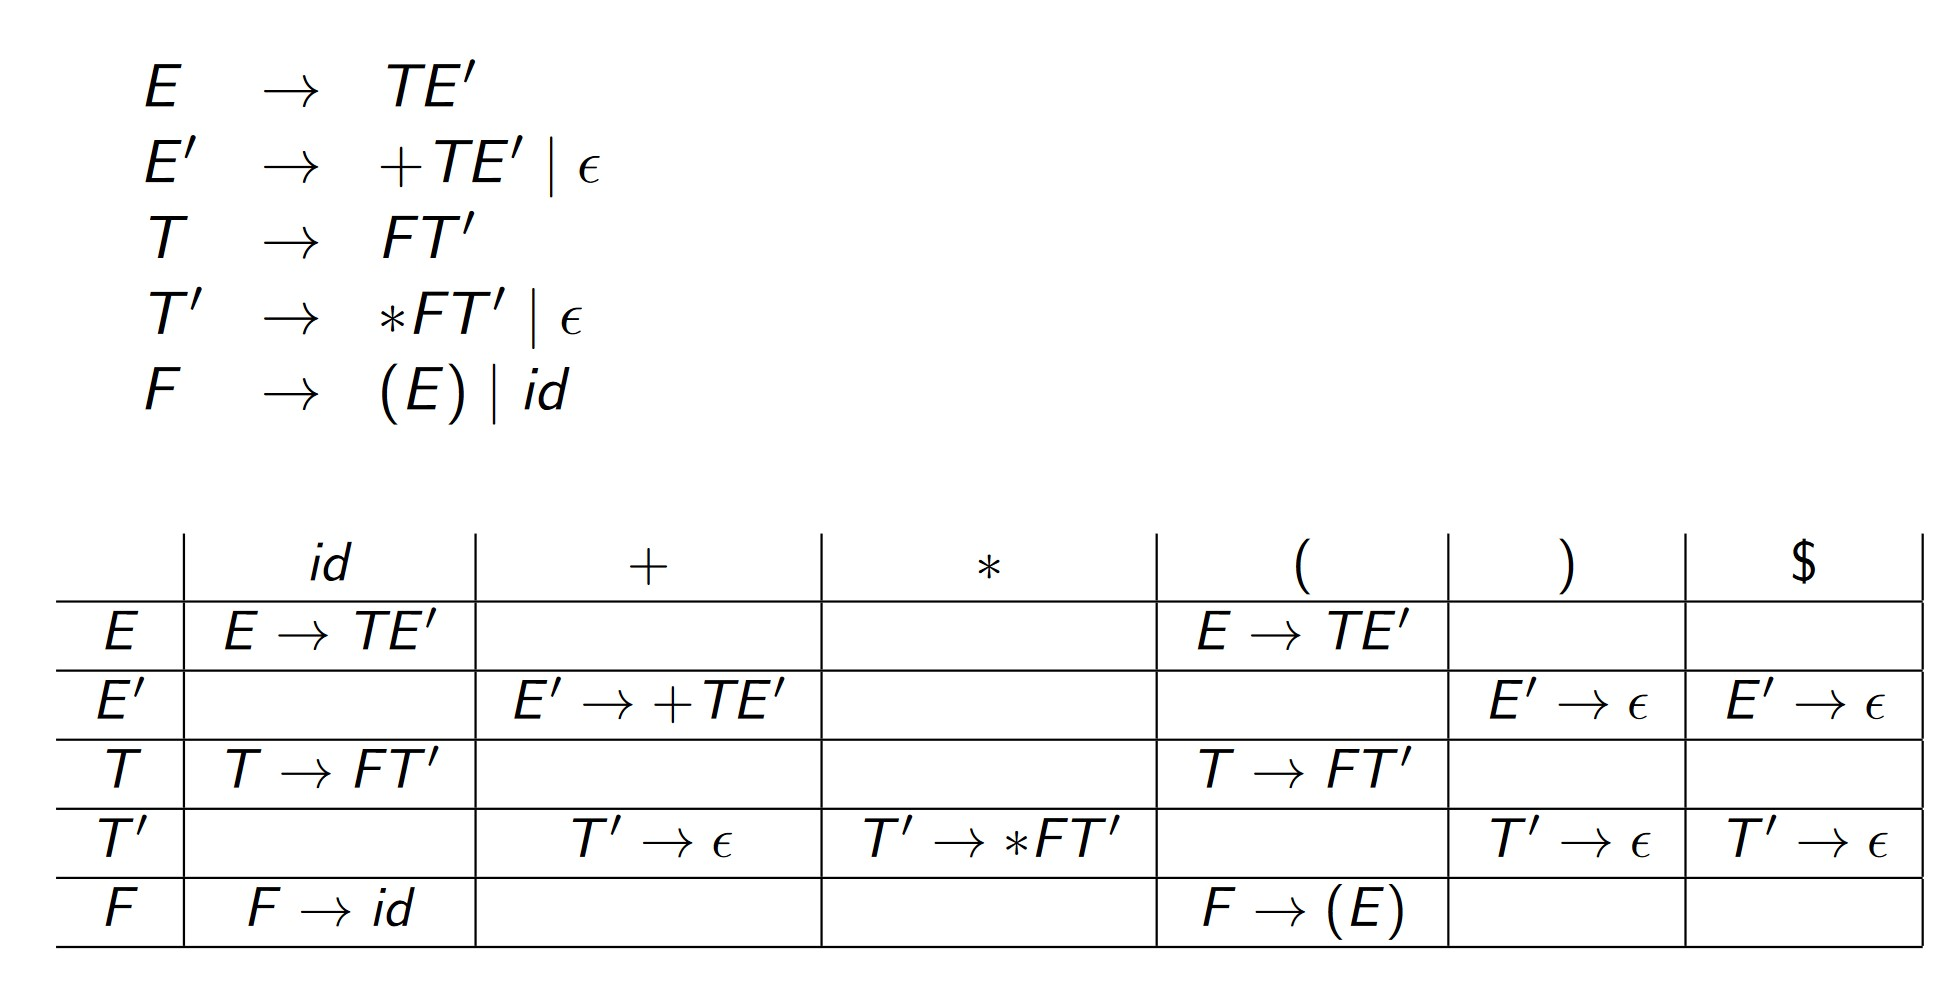
\includegraphics[width=.7\textwidth,keepaspectratio]{parsingTopDownTable.jpg}
    \caption{parsingTopDownTable}
    \label{parsingTopDownTable}
\end{figure}

La tabella è così costruita:
\begin{itemize}
    \item si ha una \textbf{riga} per ogni non-terminale della grammatica
    \item ed una \textbf{colonna} per ogni terminale della grammatica a cui si aggiunge il simbolo \$ che viene aggiunto alla parola fornita in input ed utilizzato come terminatore
    \item le entry vuote all'interno della tabella identificano i casi di errore.
\end{itemize}

Avendo a disposizione la tabella di parsing, la cui costruzione verrà trattata successivamente, è possibile utilizzarla per il parsing top-down predittivo.

\subsubsection{Algoritmo per il Predictive Top-Down Parsing}
\begin{itemize}
    \item Input: Una stringa \(w\), una tabella \(M\) di parsing top-down per la grammatica \(\mathcal{G} = (V, T, S, \mathcal{P})\)
    \item Output: La derivazione leftmost della stringa \(w \iff w \in \mathcal{L(G)}\) altrimenti \emph{error()}
    \item Inizializzazione: si posiziona \(w\$\) nell'input buffer e, nella pila che viene utilizzata per inserire ed analizzare gli elementi parziali, viene inserito il simbolo \$ con in cima \(S\) (Start Symbol)
\end{itemize}

\begin{figure}[h]
    \centering
    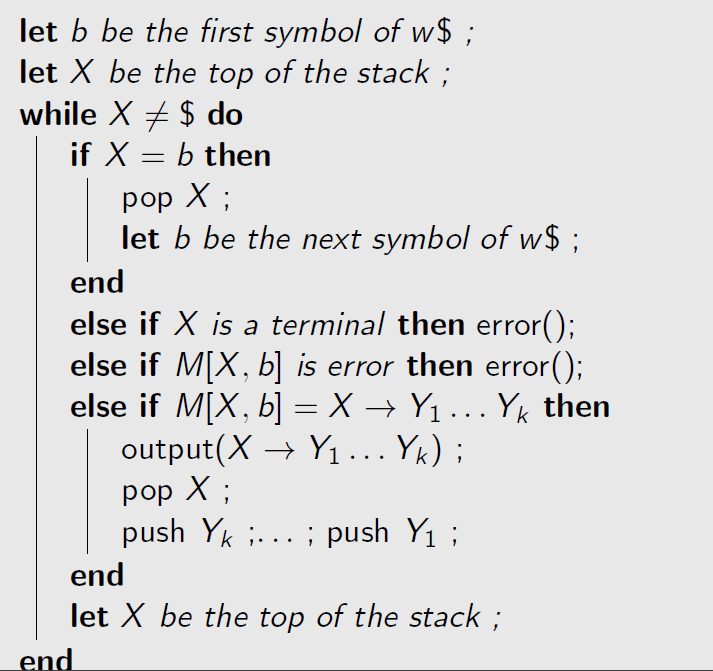
\includegraphics[width=.7\textwidth,keepaspectratio]{PredictiveTopDownAlgorithm.png}
    \caption{PredictiveTopDownAlgorithm}
    \label{PredictiveTopDownAlgorithm}
\end{figure}

Nell'algoritmo di parsing si utilizza la variabile \(b\) come primo simbolo delle parola w\$ e si inizializza la variabile X con la cima dello stack (il caso base corrisponde ad avere \(X = S\)). Finchè \(X \neq \$\) (sostanzialmente finchè non ho svuotato completamente la pila), sono dati i seguenti casi

\begin{enumerate}
    \item se \(X = b\) allora tolgo l'elemento dalla cima della pila e imposto \(b\) al simbolo successivo nell'input buffer. Questo corrisponde al caso in cui nella derivazione della costruzione parziale ho ottenuto un match con un terminale nella parola
    \item se invece X è comunque un terminale allora deve essere che \(X \neq b\) ma ciò produce un errore
    \item se invece X è un non-terminale allora è necessario verificare la tabella di top-down parsing in posizione \(M[X, b]\) e possono valere le seguenti
    \begin{itemize}
        \item \(M[X, b]\) = \emph{error} e allora viene restituito error()
        \item \(M[X, b] = X \rightarrow Y_1...Y_k\) e quindi è una produzione che verrà utilizzata per continuare la derivazione: questa viene stampata in output, viene rimosso l'elemento \(X\) dalla testa della pila e infine viene inserito il body della produzione in ordine inverso (cioè in modo che \(Y_1\) sia l'elemento in cima allo stack).
    \end{itemize}
\end{enumerate}

Infine come ultima operazione \(X\) viene assegnato all'elemento in cima alla pila e si ripete.

A seguire un esempio che fa uso dell'algoritmo appena descritto.

\begin{figure}[h]
    \centering
    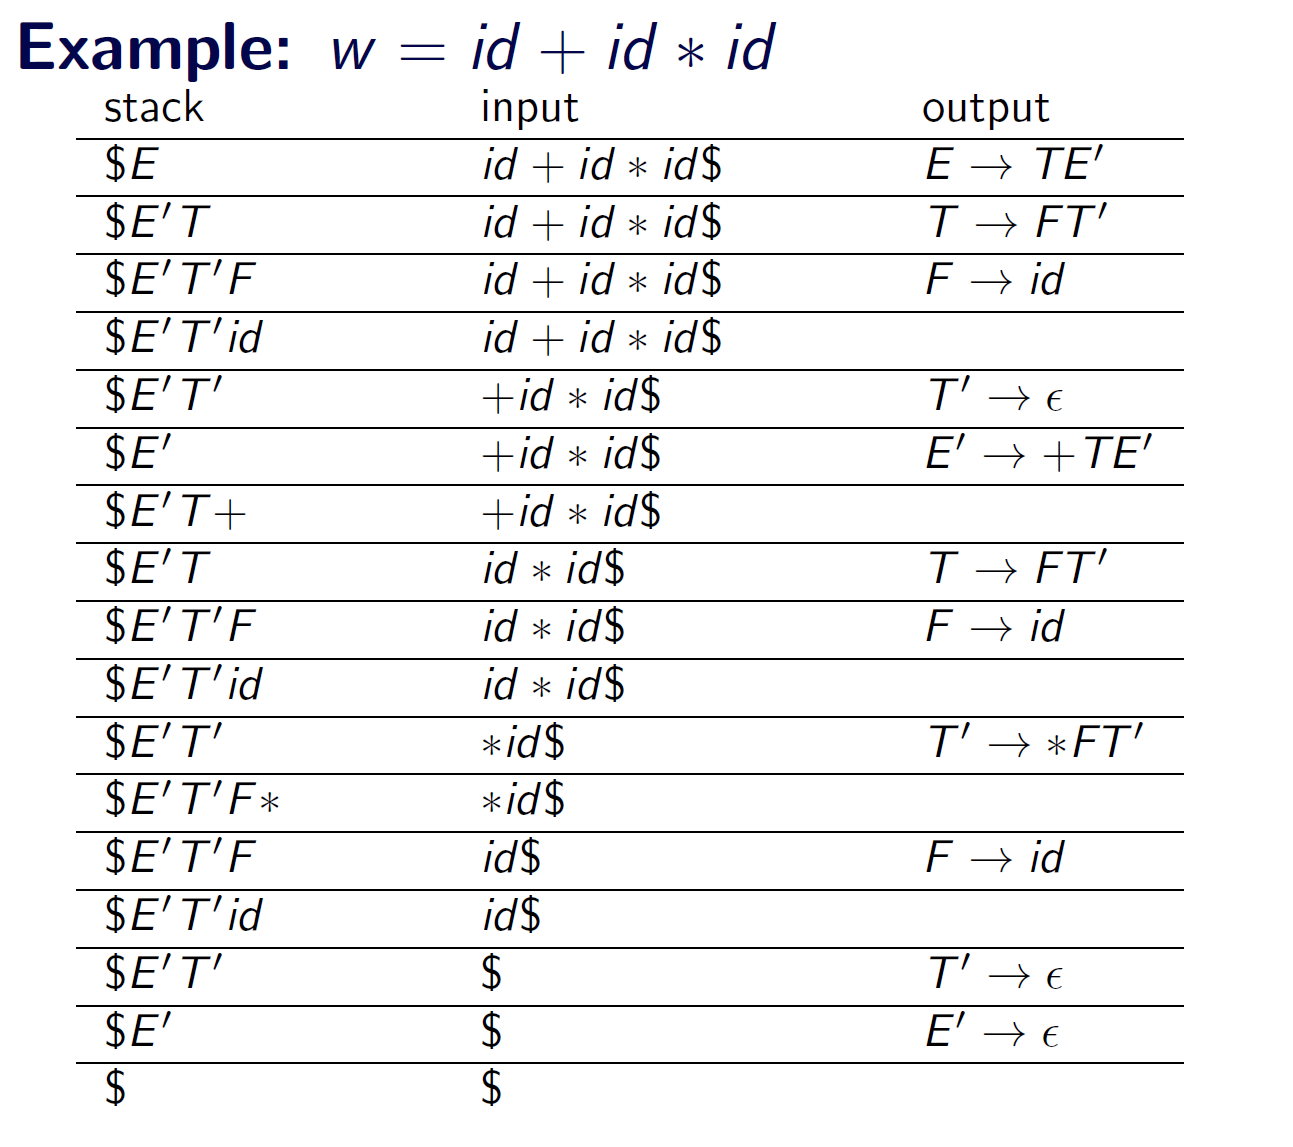
\includegraphics[width=.7\textwidth,keepaspectratio]{TopDownExercise.png}
    \caption{TopDownExercise}
    \label{TopDownExercise}
\end{figure}

\subsection{Parsing Tables}
La domanda ora è: come riempiamo la tabella? % Bella domanda ce lo dice quando ci ri-zoomiamo

\end{document}